\documentclass[a4paper,11pt,imgdir=imgs,oneside]{bthesis}
\ifdefined\printthesis
  \usepackage[print]{thesissetup}
\else
  \usepackage{thesissetup}
\fi
\title{X server in web browser}
\author{PEREZ HERNANDEZ Daniel}
% You should use waseda domain address, because you graduate Waseda University.
% For example: tuvistavie@dcl.cs.waseda.ac.jp
\email{tuvistavie@gmail.com}
\studentnb{1W09C753-8}
\supervisor{Tatsuo Nakajima}
\diploma{Bachelor in Information and Computer Science}
\date{\today}
\begin{document}
%
\frontmatter{}
%
\maketitle
%
\begin{abstract}
  Most new users to Linux have a lot of problems to set up a 
  Linux installation, which is however often necessary for students 
  in computer science. Using a remote server with already all the 
  necessary tools prepared would therefore be a good alternative, 
  but having to do everything over SSH would probably be too 
  difficult for someone who is not yet used enough to programming 
  and UNIX/Linux. The purpose of this research is to develop an X 
  server running in any web browser and able to connect to a remote 
  UNIX/Linux server, so that one could access a remote server using 
  a GUI without any need to install anything on his or her computer. 
\end{abstract}
%
\tableofcontents
%
\newpage
%
\listoffigures
%
\newpage
%
\chapter{Preface}
This report is written in partial fullfillment of the requiremenets 
for the degree of Bachelor in Computer Science. 

The project presented here is still under active development and 
will continue to be at least during the next six months. When writing 
this paper, the application is at a state where the main framework 
is operational and basic examples can be ran, but is still very far 
from being able to respond to a real world use case. The integrality 
of the project source code is available on 
\href{https://github.com/tuvistavie/scala-x-server}{GitHub} 
and under MIT license.

%
\newpage
%
\mainmatter{}
%
\chapter{Introduction}
%
\section{Motivations}
\subsection{Easy access to Linux}
From its first releases, and during several years, Linux has been quite 
complicated and not very intuitive to use (eg. no graphic installer) for beginners.
In the last few years, Linux has become much simpler to install, and use in general, 
with distributions such as Ubuntu or Fedora integrating a user friendly installer 
and even tools such as Wubi to make the installation possible from Windows.
% You should add a reference or a footnote to Wubi.

However, even if the installation process has become much simpler, the fact is that 
a lot of beginners are still having a lot of problems to get a usable Linux environment. 
While teaching C programming language as a teacher assistant, I wrote 
on my personal blog all the steps to get a usable Linux environment, using the 
possibly simplest setup: giving a disk image file to open with VirtualBox. 
Despite this, a large number of students still could not get Linux to work properly.
% You may be able to add this experience as an evaluation of the difficulty for the installation.

One of the greatest motivation for this project was therefore to create a system to 
make Linux available to anyone, even with no computer knowledge at all.
%
\subsection{Access from mobile devices}
Another interesting possibility for this project is a mobile access from any modern 
phone or tablet to a remote machine. By using this system, one could check anything,
for example the status of a running task,  on a given machine without having 
to create or use a dedicated API for it. This could be useful when the creation of 
a dedicated tool is not worth.
%
\subsection{Evaluation of new web technologies }
Web technologies have been evolving during the last few years, and a lot 
of new tools and technologies have been released. With the introduction of
websockets, a full duplex communication between a browser and a web server 
have become possible. 
The last motivation for this project was to try and evaluate these new web 
technologies, in particular websockets, to see how well it can be integrated 
in a resource demanding project.


%
\section{About X protocol}
The whole application is using the X protocol
\footnote{\url{http://www.x.org/docs/XProtocol/proto.pdf}}, 
we are therefore going to give a brief presentation of this protocol, 
for the reader to be able to understand the concepts in this paper.
\subsection{Generalities}
The X protocol is a network-transparent protocol for bitmap display. 
It uses a client-server architecture, running the server on the computer 
with the display, and makes the connection with local and remote clients possible. 
It is a binary protocol and can be built on top of any reliable byte stream (eg. TCP).
\subsection{Messages}
The protocol uses four main types of messages to communicate between 
the server and the clients. Those types are
\begin{description}
\item[Requests] A request is the basic way to communicate from the client 
  to the server and can be used either to query for some information or to 
  update the display. Some requests need a reply while other do not. 
  Requests needing a reply can be asyncrhonous or not.
\item[Replies] A reply is the basic way for the server to send back
  information to the client, and is usually used to send information about the server.
\item[Events] Events are generated by the server and sent to the client to notify it of 
  some event in the handled display. Event can be used for graphic events 
  (eg. when a window has been rendered) or for device events (eg. keyboard or mouse event).
\item[Errors] Errors can be generated from the client as well as the server
  for many different reasons. One of the main reason for errors generated 
  from the server side is for access to non available resources.
\end{description}
An overview of how these messages are sent is shown in figure~\ref{fig:xcore-overview}.
\begin{figure}[tb]
  \begin{center}
    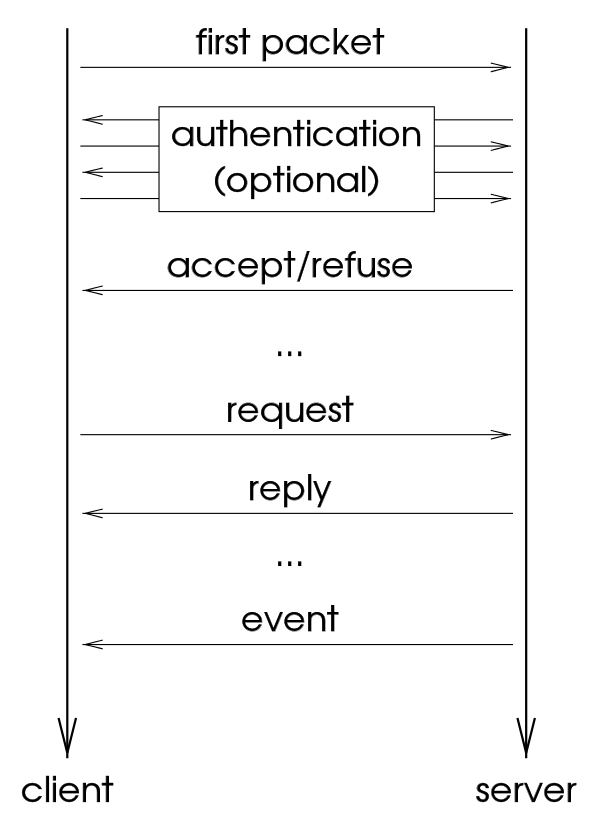
\includegraphics[height=8cm,width=6cm]{imgs/xcore-overview.png}
    \caption{\label{fig:xcore-overview}Overview of the X protocol \protect\footnotemark}
  \end{center}
\end{figure}
\subsection{Resources}
The protocol uses a number of different resources which we will shortly 
introduce here.
\begin{description}
\item[Drawable] A drawable is an abstract entity used to draw. It can be a window or a pixmap.
\item[Window] There are two types of window: top-level window and subwindows. 
  A top-level window is the main container for an application and 
  usually contains all the other components of the application.
  A subwindow is a window contained in the top-level window of an application 
  and can be used for anything, from the titlebar to a button in the application.
\item[Pixmap] A pixmap is a region used to draw, but on opposite to a window, 
  it is not shown until explicitly requested. The content of a pixmap 
  or part of it can be displayed on a window.
\item[Graphic context] A graphic context is a structure containing basic graphic 
  information to apply to a given request, for example the background and 
  foreground colors, or a transformation to apply to the shape to draw.
\footnotetext{Diagram from Wikipedia \href{http://en.wikipedia.org/wiki/X_Window_System_core_protocol}{X Window System Core Protocol}}
\subsection{Short example}
To end up with the presentation of the X protocol, we will here give a
short example of a communication between an X server and an X client.
\end{description}

%
\section{About the project}
We will here be giving a short overview of what was tried in this project, 
what can be done and what still needs to be done.
\subsection{Achieved tasks}
One of the main task of this project was to make a communication possible 
between an X client and a modern browser. This is now possible and though 
not all X requests and events are supported yet, they can be added 
simply enough.
A simple application can already be ran using the system, although the 
number of supported requests and replies is still very limited.
\subsection{Tasks to be achieved}
Still only very few requests, replies and events are supported by the 
actual system. In order to be able to respond to real world requests, 
not only those requests will be needed, but some requests and 
other messages that are not defined by the core X protocol will 
be needed. We are now working on extending the base system to support 
these messages, but given the number of message that must be handled, 
the stable release of these is going to take some time.
%
\chapter{About X protocol}
The whole application is using the X protocol
\footnote{\url{http://www.x.org/docs/XProtocol/proto.pdf}}, 
we are therefore going to give a brief presentation of this protocol, 
for the reader to be able to understand the concepts in this paper.
\section{Generalities}
The X protocol is a network-transparent protocol for bitmap display. 
It uses a client-server architecture, running the server on the computer 
with the display, and makes the connection with local and remote clients possible. 
It is a binary protocol and can be built on top of any reliable byte stream (eg. TCP).
\section{Messages}
The protocol uses four main types of messages to communicate between 
the server and the clients. Those types are
\begin{description}
\item[Requests] A request is the basic way to communicate from the client 
  to the server and can be used either to query for some information or to 
  update the display. Some requests need a reply while other do not. 
  Requests needing a reply can be asyncrhonous or not.
\item[Replies] A reply is the basic way for the server to send back
  information to the client, and is usually used to send information about the server.
\item[Events] Events are generated by the server and sent to the client to notify it of 
  some event in the handled display. Event can be used for graphic events 
  (eg. when a window has been rendered) or for device events (eg. keyboard or mouse event).
\item[Errors] Errors can be generated from the client as well as the server
  for many different reasons. One of the main reason for errors generated 
  from the server side is for access to non available resources.
\end{description}
An overview of how these messages are sent is shown in figure~\ref{fig:xcore-overview}.
\begin{figure}[tb]
  \begin{center}
    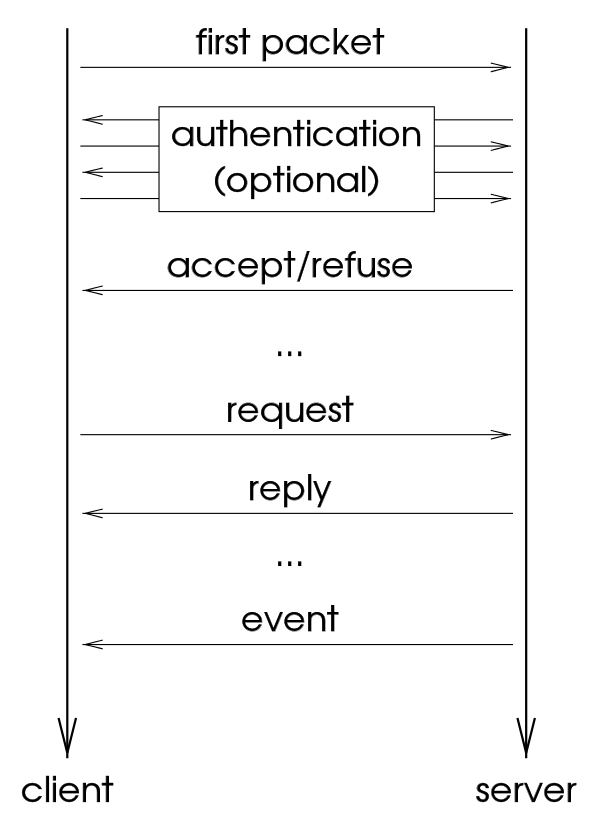
\includegraphics[height=8cm,width=6cm]{imgs/xcore-overview.png}
    \caption{\label{fig:xcore-overview}Overview of the X protocol \protect\footnotemark}
  \end{center}
\end{figure}
\section{Resources}
The protocol uses a number of different resources which we will shortly 
introduce here.
\begin{description}
\item[Drawable] A drawable is an abstract entity used to draw. It can be a window or a pixmap.
\item[Window] There are two types of window: top-level window and subwindows. 
  A top-level window is the main container for an application and 
  usually contains all the other components of the application.
  A subwindow is a window contained in the top-level window of an application 
  and can be used for anything, from the titlebar to a button in the application.
\item[Pixmap] A pixmap is a region used to draw, but on opposite to a window, 
  it is not shown until explicitly requested. The content of a pixmap 
  or part of it can be displayed on a window.
\item[Graphic context] A graphic context is a structure containing basic graphic 
  information to apply to a given request, for example the background and 
  foreground colors, or a transformation to apply to the shape to draw.
\footnotetext{Diagram from Wikipedia \href{http://en.wikipedia.org/wiki/X_Window_System_core_protocol}{X Window System Core Protocol}}
\section{Example}
To end up with the presentation of the X protocol, we will here give a
short example of a communication between an X server and an X client.
\end{description}

%
%You should add related works.
%
\chapter{General architecture}
%
% One sentence is too long.
In this project, everything is based on the X protocol, but given the 
requirements of the system, there are a lot of things that needed to be 
handled in alternative ways, and the core X protocol has only remained 
in the backend of the system, while the other parts and especially the 
frontend used in the browser is relying on much more modern technologies.

We will here discuss about the general architecture of this project, 
including the differences with the basic X protocol as well as their 
reason to be.
%
\section{General overview}
We will here be giving a general overview of the project. 

The project is mainly divided in three different parts, and the general 
communication pattern is shown in figure~\ref{fig:project-overview}.
\begin{figure}[tb]
  \begin{center}
    \begin{tikzpicture}[
  system/.style={draw,rectangle,rounded corners=3,minimum width=2cm,text width=1.8cm,text centered},
  node distance=2cm
  ]
  \draw (-7, -2.5) rectangle + (10,3.5);
  \draw (-6, -3) node  {Remote computer};
  
  \draw (-1.5, -6.3) rectangle + (3,1.5);
  \draw (2.8, -4.5) node {Local machine};

  \node[system] (sf) {Server front app};
  \node[system, below=4.8cm of sf] (fe) {Front end};
  \node[system, left=3.5cm of sf] (sb) {Server back app};
  \node[system, below=1cm of sb] (xc) {X client};

  \draw[style={->,>=triangle 45}] 
  ($(sb.east)+(0,-0.3)$) -- 
  ($(sf.west)+(0,-0.3)$)
  node [midway, below] {Transfer requests};
  
  \draw[style={->,>=triangle 45}] 
  ($(sf.west)+(0,0.3)$) --
  ($(sb.east)+(0,0.3)$)
  node [midway, above] {Transfer data};

  \draw[style={->,>=triangle 45}]
  ($(sb.south)+(-0.4,0)$) -- 
  ($(xc.north)+(-0.4,0)$);
  
  \draw[style={->,>=triangle 45}] 
  ($(xc.north)+(0.4,0)$) -- 
  ($(sb.south)+(0.4,0)$);

  \draw[style={->,>=triangle 45}]
  ($(fe.north)+(-0.5,0)$)--
  ($(sf.south)+(-0.5,0)$)
  node [midway, left, align=right] {Replies\\Events};
  
  \draw[style={->,>=triangle 45}] 
  ($(sf.south)+(0.5,0)$) --
  ($(fe.north)+(0.5,0)$)
  node [midway, right, align=left] {Requests};
\end{tikzpicture}
    \caption{\label{fig:project-overview}System general communication pattern}
  \end{center}
\end{figure}
\begin{description}
\item[Server backend]
  This application main role is to communicate with the X clients, 
  to transfer the requests sent by the X clients to the frontend fo the system, 
  and to transfer back the replies and events sent by the frontend to the 
  X clients. 
  
  Another important role of this application is to store as possible 
  the information held by the client and the frontend in order to, whenever 
  possible avoid unneeded communication by responding directly without 
  needing to transfer any information.

  To illustrate this caching system, let us think about a requests sent by a 
  client to get the background and foreground pixels of a particular 
  subwindow (the root window information being sent on connection). If the 
  backend server was doing any cache work, the request would have to be 
  sent to the frontend application, and then to the client web browser, before 
  getting an answer, which would result in a, depending on the bandwith, 
  quite long latency for a very basic request.   
  
\item[Server frontend]
  One of the roles of this application  is to act as a bridge to
  communicate between the backend application of the system 
  and the web browser JavaScript application.

  Another of its role is to act as a login manager. The application 
  receives an HTTP request with the client Linux/UNIX creditentials 
  check those creditentials, and on success, initializes the server 
  backend for the particular client as well as the websocket connection 
  to communicate with the web browser.
\item[Web browser application]
  The web browser application is the application running in the client 
  browser, and has several responsibilities in the system.

  The first responsibility of this application is to handle the 
  requests received from the server and to render them in the web 
  browser.
\end{description}




%
\section{Differences with a normal X server}
In this section, we will discuss between the main differences of this project 
with a normal X server.
\subsection{Divided server}
In a normal X client/server architecture, the client connects to the server, 
and communicates directly with it. The X server needs to have control over the 
keyboard, mouse, screen, and other hardware used to display graphics, and handle events.

This system is very different as first of all, there is not really \emph{an} X server.
Given the system requirements, the application that communicates with the client and the 
application that listens to the events cannot be the same; handling all the TCP 
directly in the web browser is not realistic. There is therefore a need 
to communicate with clients, and make communication possible with the application 
acting as the X server frontend.
%
\subsection{Communication through websockets}
As a consequence of the above difference, another difference is that to 
implement this system, we need not only to communicate with X clients using 
a bytestream such as TCP sockets, but we also need to use some communication protocol to 
communicate with a web browser. The chosen protocol to achieve this is 
websockets, we will be discussing further about this decision later in 
this paper.
%
\subsection{Integrated login manager}
This project goes further from a normal X server in the sense that the 
login manager is integrated and therefore does not depends on the 
X Display Manager Control Protocol.
%
\section{Language and tool choice}
%
The web browser application is written in JavaScript, and we made the 
choice to avoid any DOM libraries that could potentially slow down the application.
The application however does use KineticJS\footnote{\url{http://www.kineticjs.com/}}
for rendering.
%
The application running on the server has been almost entirely developed in Scala. 
In this section, we will try to discuss objectively a little about 
the motivations for choosing this language.
%
\subsection{Multi-threading}




%
\chapter{Server frontend application}
%
%
\chapter{Server backend application}
%
The server backend is the part of the system that communicates directly with the X clients, 
and takes care to transfer the necessary requests to the frontend application, as well as 
transferring back the replies and events sent from the frontend.

Another important point about this application is that it caches the information received 
from the X client and back from the frontend application, and using this cache tries to
handle requests coming from the X client locally, without transferring them when not needed.

We will here discuss about how this application is designed and implemented.
%
\section{General explanations}
%
We will here describe the general working of the backend application. % This sentece may be verbosity.

% I recommend that below sentence is divided into multiple sentences.
The application is launched asynchronously from the frontend application, 
therefore, when starting up the backend application first sends a message to 
the frontend to let it know that the application is now started and ready to 
receive and transfer messages. This is a single-way communication and the 
application does not wait for any answer from the frontend.

The second step when starting up the backend is to start listening on the 
port the X clients will be connecting to. The hostname 
to listen is statically set using a configuration file, however as the port 
to listen to changes depending on the current screen number, the port number to 
use to listen for incoming connection is sent as a command-line argument of the 
application. Typically, the first application to start will be given the 
screen number $0$, and will therefore be listening on the port $6000$ 
(see~\ref{ssec:connection-setup}).
% What port number is assigned to Second and Third request?

Finally, the application reads the initialization file of the current user 
to start launching applications (eg. a window manager or desktop environment). 
This file should be placed in the user home directory, and is called 
\lstinline{.scalaxsrc}, however we plan to use the file \lstinline{.xinitrc} to 
try to imitate the behavior of \lstinline{startx}
\footnote{\href{http://linux.die.net/man/1/startx}{\lstinline{startx}} is a script used to start the X Window System.}
or SLiM
\footnote{\href{http://slim.berlios.de/}{SLiM (Simple Login Manager)} is a graphical login manager for X.}.

Once the application have finished initializing, it should received the first requests 
from X clients launched when reading the initialization file.

When a request is received, the information given by the request, if any, is cached 
by the application, and the request is handled locally when possible, otherwise 
transferred to the frontend application. We will discuss about this further in the next 
section.

To handle requests sent by the X clients, the application first parses the requests and 
transforms it in a normal Scala object. It then checks if the requests needs to be handled 
locally, if the content of the requests needs to be cached, and finally if the request 
needs to be transferred to the frontend and sends it to the frontend through a TCP connection 
when needed.

%
\section{Caching}
%
As said in the previous section, an important responsibility of the backend application is to
cache data received by both the X clients and the frontend application, and to use this cache 
efficiently to try to reduce the most possible the requests and replies transfers to the 
frontend application.

The caching system has not yet been implemented in the system when writing this paper, but the 
strategy to use is straightforward and should not be too difficult to implement.

The first step is to check if the requests content needs to be cached or not. 
As the requests are implemented as Scala case classes, we could easily add a trait 
to the requests that need to be cached. A possible example of this implementation is shown 
in listing \ref{list:caching}.

\begin{lstlisting}[basicstyle=\footnotesize,caption=Possible implementation of requests needing cache,language=scala,label=list:caching]
trait NeedsCaching { // define trait for caching
  def cacheRequest(): Unit
}

// mixin traits to class needing to be cached
case class CreateWindowRequest (
 ...
) extends Request 
  with NeedsTransfer // needs to be transfered to the frontend
  with NeedsCaching { // needs to be cached 
  ...
  def cacheRequest() {
    // do caching logic
  }
}

// handle requests needing caching
request match {
  case r: NeedsCaching => r.cacheRequest()
  ...
}
\end{lstlisting}
Of course, the listing above is quite minimalist, but this should be enough to check if requests need 
caching and handle them. 

The content of the \lstinline{cacheRequest} method being too different 
for each request, we will not enter in the possible implementation details here, but at least 
for the different resources, the idea would be to save them as an appropriate model instance 
after checking that the resource id is valid.

Using this method, the errors of access to unavailable could be done in the backend application 
without any need to transfer the request further.

%
%
\chapter{Web browser application}
%
The web browser application is the interface through which the user connects to the system 
and then controls it. It receives messages from the server frontend application and renders them 
on the browser screen. It also handles the browser's events and transfer them to frontend
application.
%
\section{Rendering}
%
As mentioned above, the first role of the application is to render the requests received from 
the frontend application, and therefore indirectly from the X client running for the user's 
X session. Listing~\ref{list:sample-request} shows a sample request that is received 
through the websocket channel and rendered by the application.
\begin{lstlisting}[basicstyle=\footnotesize,caption=Sample request,language=javascript,label=list:sample-request]
{
  "type":"request",
  "content": {
    "clientId": 1,
    "opCode": 70,
    "action": "PolyFillRectangleRequest",
    "request": {
      "drawable": 4194305,
      "context": 4194304,
      "rectangles": [{"x":20,"y":20,"width":200,"height":200}]
    }
  }
}
\end{lstlisting}
The object contained in the \lstinline{request} key is almost exactly the request 
sent by the X client to the backend application, translated in JSON, except from the 
op-code being stored in the wrapping object to make the request easier to handle.
The rest of the message is extra meta information to help the browser handling 
requests efficiently. 

The rendering implementation is based on KineticJS, and each window is treated as 
a different layer so that refreshing the display can be done without having to 
draw again the whole screen. This rendering strategy improves a lot performance as the
area to redraw for each request is only the given part of the window and the rest of 
the display can stay intact.

%
\section{Event handling}
%
The next of this application is event handling, however, the implementation of this 
functionality not being done yet, we will here only give a general overview of the 
approach that will be taken to implement it.

The event that are to be handled by the X server are decided by the X client, 
and are different for each window.

The windows are created as KineticJS groups, and 


%
%
\chapter{Conclusion}
\section{Discussion and future work}
The evaluation of the system has not been possible as the system implementation have not gone far enough yet.
There are a lot of points that need further confirmation, and a we will
especially need to check performance in a real use-case, to see 
if the system could actually be used responding to real-world requirements.

Some unsolved problems still remain, such as truetype fonts handling, 
or large data transfer. Truetype fonts could be rendered as drawings using 
Canvas
\footnote{The \href{http://typeface.neocracy.org/}{Typeface} project seems to be able to render truetype fonts using Canvas.}
. Large data transfer could be done opening another websocket channel 
to avoid blocking the main communication channel especially when the 
connection is slow.

This project will continue to be developed, and we will try to reach 
a real-world usable implementation in the next six months.
\section{Final words}
Though a lot of work still needs to be done, we have managed to 
build a system to use a Linux/UNIX machine from a web browser 
using the X protocol. 

From this experience, we could actually showed that new web technologies 
offer a lot of new possibilities, and we will try to continuing to prove it 
while continuing the project.
%
\appendix{}
%
\chapter{Actor model}
%
%
\backmatter{}
%
\refstepcounter{chapter}
%
\bibliographystyle{plain}
\addcontentsline{toc}{chapter}{\bibname}
\nocite{*}
\bibliography{main_bibliography}

\end{document}
